\documentclass[xcoler=dvipsnames, aspectratio=169]{beamer}

\usepackage{3191Style}
\newcommand{\C}{\mathbb{C}}
\newcommand{\F}{\mathbb{F}}
\newcommand{\abs}[1]{\left|#1\right|}
% Date gives the title of the lecture
\date{Orthogonal Projection}

\begin{document}
    \begin{frame}{Orthogonal Projection} % Have an image here
        \begin{center}
            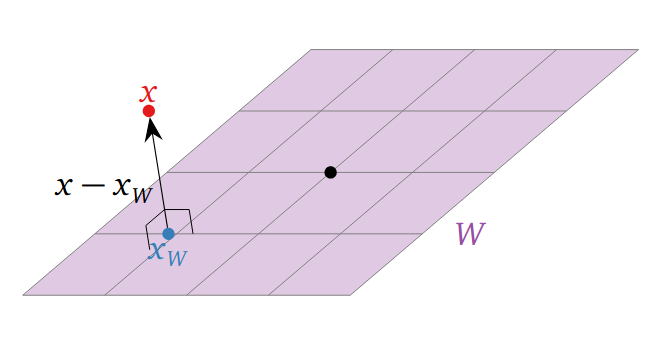
\includegraphics[width=.3\textwidth]{images/orthProj.png}
        \end{center}
        In some applications, we have a vector $\vec{x}$ that's not in a space we want, and can sometimes
        be content with the ``closest'' vector to $\vec{x}$ that lives in our space $W$.\pause
        \begin{defn}
            \rText{Orthogonal Projection}: We call this vector $\vec{x}_W$ to be the \bText{orthogonal
            projection} of $\vec{x}$ onto the space $W$.
        \end{defn}
    \end{frame}
    \begin{frame}{Why call it Orthogonal? An $\R^2$ Figure}
        \begin{columns}
            \column{.5\textwidth}
                \begin{center}
                    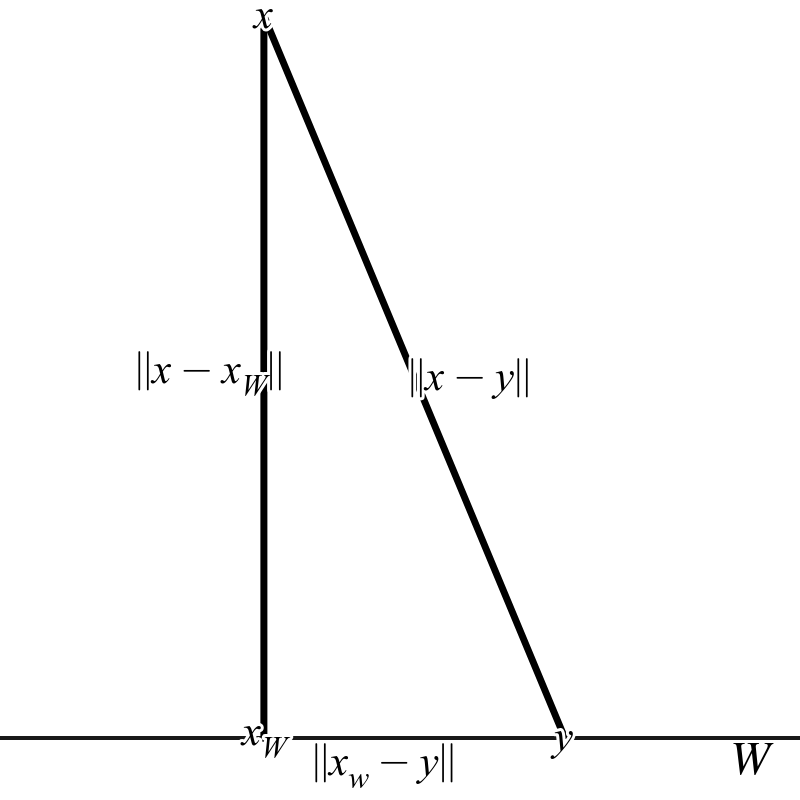
\includegraphics[height=.8\textheight]{images/orthProjEx2.png}
                \end{center}
            \column{.5\textwidth}
            If we take any other point as $\vec{x}_W$, then we see that it would be further from 
            $\vec{x}$.\pause\ See that the vector $\vec{x}-\vec{x}_W$ is orthogonal to $W$!
        \end{columns}
    \end{frame}
    \begin{frame}{Orthogonal Decomposition}
        Let's suppose we can compute this $\vec{x}_W$, and note something.\pause
        \begin{defn}
            \rText{Orthogonal Decomposition}:
            Let $W$ be a subspace of $\R^n$, and $\vec{x}\in\R^n$. Then, we can write $\vec{x}$
            as\pause
            \[
                \vec{x} = \vec{x}_W + \vec{x}_{W^\perp}
            \]\pause
            This is called the \bText{orthogonal decomposition} of $\vec{x}$. Where $\vec{x}_W$ is
            the orthogonal projection of $\vec{x}$ onto $W$ and $\vec{x}_{W^\perp} = \vec{x}-\vec{x}_W$
        \end{defn}
    \end{frame}
    \begin{frame}{Computing an Orthogonal Projection}
        \begin{theorem}
            Let $A\in\R^{m\times n}$, $W = \colS{A}$, and $\vec{x}\in\R^{m}$. Then the system of
            linear equations given by
            \[
                A^\top A\vec{c} = A^\top\vec{x}
            \]
            is consistent and $\vec{x}_W = A\vec{c}$ where $\vec{c}$ is some solution.
        \end{theorem}\pause
        \emph{Note}: We sometimes call this equation the ``normal equations'', which is particularly
        important for statistics applications when finding covariances of random variables.\pause\

        Note that if $n=1,$ then we have inner products instead of matrix multiplications!
    \end{frame}
    \begin{frame}{Finding Orthogonal Projection Example}
        \small
        Let $W = \Span{\bMat{1\\0\\-1}, \bMat{1\\1\\0}}$. Find an orthogonal projection of
        $\vec{x} = \bMat{2\\1\\4}$\pause\\ We will first solve $A^\top A\vec{c} = A^\top\vec{x}$\pause
        \[
            A^\top A\pause = \bMat{
                1 & 0 & -1\\
                1 & 1 & 0
            }\bMat{
                1 & 1\\
                0 & 1\\
                -1& 0
            }\pause = \bMat{
                2 & 1\\
                1 & 2
            }\pause\qquad A^\top\vec{x}\pause = \bMat{
                1 & 0 & -1\\
                1 & 1 & 0
            }\bMat{2\\1\\4}\pause = \bMat{-2\\3}
        \]
        \[
            \aMat{c|c}{
                A^\top A & A^\top\vec{x}
            }\pause = \aMat{cc|c}{
                2 & 1 & -2\\
                1 & 2 & 3
            }\pause\xrightarrow{R_2=R_2-\frac{1}{2}R_1}\aMat{cc|c}{
                2 & 1 & -2\\
                0 & \frac{3}{2} & 4
            }\pause\xrightarrow{R_1=R_1-\frac{2}{3}R_2}\aMat{cc|c}{
                2 & 0 & -\frac{14}{3}\\
                0 & \frac{3}{2} & 4
            }
        \]
        \vspace{-5pt}
        \[
            \pause\xrightarrow[R_2=\frac{2}{3}R_2]{R_1=\frac{1}{2}R_1}\aMat{cc|c}{
                1 & 0 & -\frac{7}{3}\\
                0 & 1 & \frac{8}{3}
            }\pause\qquad \vec{x}_W = A\vec{c}\pause = \frac{1}{3}\bMat{
                1 & 1\\
                0 & 1\\
               -1 & 0
            }\bMat{-7\\8}\pause = \frac{1}{3}\bMat{
                1 \\ 8 \\ 7
            }
        \]
    \end{frame}
    \begin{frame}{Finding Orthogonal Projection Practice}
        Let $W = \Span{\bMat{1\\0\\-1}, \bMat{1\\1\\0}}$. Find an orthogonal projection of
        $\vec{x} = \bMat{1\\2\\4}$
        \iftoggle{showSolutions}{
            \pause
            \vspace{30pt}
            \[
                \vec{x}_W = \bMat{0\\3\\3}
            \]
            \vspace{50pt}
        }{\vspace{130pt}}
    \end{frame}
    \begin{frame}{Orthogonal Projection as a Linear Transformation}
        Let's define this orthogonal projection to be the transformation $T$.
        \[
            T:\R^n\rightarrow W\qquad T(\vec{x}) = \vec{x}_W
        \]\pause\vspace{-30pt}
        \begin{theorem}
            $T$ is a linear transformation
        \end{theorem}\pause
        \vspace{-10pt}
        \begin{proof}
            We will show that for any $\vec{x},\vec{y}\in\R^n$ and $a\in\R$, we have that
            $T(a\vec{x} + \vec{y}) = aT(\vec{x}) + T(\vec{y})$.\pause\ For our convenience, we
            define $\vec{z} = a\vec{x} + \vec{y}$.\pause\
            Remember that $\vec{z}_W = A\vec{c}_z$ where $\vec{c}_z$ is a solution to 
            $A^\top A\vec{c}_z = A^\top\vec{z}$, and similarly for $\vec{x},\vec{y}$,\pause\, 
            so we need only show that $\vec{c}_z = a\vec{c}_x + \vec{c}_y$ is a solution to our 
            system above.
            \[
                A^\top A\vec{c}_z\pause = A^\top A(a\vec{c}_x + \vec{c}_y)\pause = 
                aA^\top A\vec{c}_x + A^\top A\vec{c}_y\pause = aA^\top\vec{x} + A^\top\vec{y}
                \pause = A^\top(a\vec{x} + \vec{y})\pause = A^\top\vec{z}
            \]
        \end{proof}
    \end{frame}
    \begin{frame}{Properties of Orthogonal Projection}
        Let $T$ be our orthogonal projection as defined in the previous slide, then the following properties
        are true
        \begin{enumerate}
            \pause\item $T(\vec{x}) = \vec{x}$ if and only if $\vec{x}\in W$
            \pause\item $T(\vec{x}) = \vec{0}$ if and only if $\vec{x}\in W^\perp$
            \pause\item $T\circ T = T$
            \pause\item $T$ is surjective.
        \end{enumerate}
    \end{frame}
\end{document}
